\documentclass[english,11pt,a4paper]{article}
\usepackage{preamble}

%-------------------------------------------------------------------------%
% MASTERARBEIT (╯°□°)╯︵ ┻━┻       ┬─┬ノ( º _ ºノ)      (ノಠ益ಠ)ノ彡┻━┻   %
%-------------------------------------------------------------------------%
\begin{document} %------------   \(◕ ◡ ◕\)   -----------------------------%
% (/◔ ◡ ◔)/   ◕‿◕

Version 4 \scriptsize \hfill Juri; Hyperelliptic Curves --- Draft --- \today
\normalsize

\section{Addition Law}

\subsection{Definitions and Notation}

\begin{defin}
	Let $K$ be a field with char$(K) \neq 2, 3$ and $\bar K$ its algebraic closure. Define the hyperelliptic curve of genus two $\enk$ as the set of solutions in $K^2$ to the equation $y^2=C(x)$ where $C(x)=x^5+ax^4+bx^3+cx^2+dx+e$ is a polynomial over $K$. Similarly, the set of solutions in the closure would be denoted $\enkb$.	Define $\ek$ as $\enk \cup \{ \infty \}$.

	\textbf{Note} that we could obtain a more reduced form of $C(x)$, eliminating $a$ by shifting $x$ to $x-a/5$. However, since this would rob us of the possibility of char$(K) = 5$ without simplifying our coming calculations in any significant manner, we shall be reluctant towards using this trick.

	For the purpose of clarity, let points on the hyperelliptic curve --- in the sense of solutions to $y^2=C(x)$ --- be designated by the calligraphic letter $\q=(x,y) \in \enkb$. The point opposite to $\q$ will be written $\bar \q = (x,-y)$ and by symmetry of the curve in $y$ also belongs to $\enkb$. In the case where $\q = \infty$, define $\bar \q = \infty$. %We allow ourselves to write $\pm \q$ whenever we mean in fact `either $\q$ or $\bar \q$'.

	We want to consider the set of all pairs $(\q_1,\q_2)$ and tame it with an equivalence relation with the goal of obtaining an additive group:
\end{defin}
% \vspace{2mm}
\begin{defin}\label{defj}
	Define $\J$ to be the set\scalebox{1.3}{ $\nicefrac{ \j }{\sim }$ }where $\j = \ekb \times \ekb$. It is called the ``Jacobian'' and the equivalence relation is defined by
	\begin{align*}
		(\q_1,\q_2) &\sim (\q_2,\q_1) \\
		\text{and\hspace{5mm}} (\q,\bar \q) & \sim ( \infty , \infty ). 
	\end{align*}
	Write $\{ \q_1,\q_2 \}$ from now on and let bold letters denote points on the curve in the sense of classes of unordered pairs $\P =\{ \q_1, \q_2 \} \in \J$. The point $\{ \bar \q_1, \bar \q_2 \}$ will be called $\bar \P$ for now but can already tentatively be thought of as $-\P$. Call $\{ \infty, \infty \}$ the zero of our set. Call $\q_i$ a point-component.% We will also permit ourselves the notation $\{ \q,\bar \q \} = 0$ and we refrain from explicitly stating that $\P$ is in fact an equivalence class.

	A point $\q = (x_0,y_0)$ is called singular if it fulfills both $y_0=0$ and $C'(x_0) = 0$. A curve is called singular if and only if it has a singular point. We consider only non-singular hyperelliptics from here on; this amounts to $C(x)$ having no repeated factors over $\bar K$ (``squarefree)''.%xxx
\end{defin}

\subsection{The General Case}

Let $\P_1 = \{\q_1,\q_2\}$, $\P_2 = \{\q_3,\q_4\}$ with $\q_i = (x_i,y_i) \in \enk$ or $\q_i = \infty$. To define $\P_3 = \P_1 + \P_2$ we distinguish between one general case and a number of special cases and first derive the results of the former before enumerating the latter ones.

\begin{case} {\scshape Four Distinct Point-Components:}
	Let first $\q_i \in \enk$ and $\P_i$ be defined as above with $x_i \neq x_j$ whenever $i \neq j$.

	The overarching idea is to obtain a fifth and sixth $x$-coordinate and the corresponding $y$-coordinates by passing a polynomial of degree three through the four points $\q_i$. Ideally this should give us two additional intersections with the curve which we then use as the components of our point $\P_1 + \P_2$.

	{\scshape Step 1:} It is known that the Vandermonde matrix
	\begin{align*}V=
		\begin{pmatrix}
			1 & x_1 & x_1^2 & x_1^3\\
			1 & x_2 & x_2^2 & x_2^3\\
			1 & x_3 & x_3^2 & x_3^3\\
			1 & x_4 & x_4^2 & x_4^3\\
		\end{pmatrix}
	\end{align*}
	has determinant $\prod_{i < j} (x_i-x_j)$ which is conveniently non-zero if and only if the $x_i$ are pairwise distinct. Let $p(x) = p_3 x^3 + p_2 x^2 + p_1 x + p_0 \in \bar K[x]$ be the polynomial in unknown coefficients that we are looking for. With $\textbf{y} = (y_1 \ y_2 \ y_3 \ y_4)^t$ and $\textbf{p} = (p_0 \ p_1 \ p_2 \ p_3)^t$, the problem of determining $p(x)$ can be rewritten as
	\begin{align*}
		V \cdot \mathbf{p} = \mathbf{y}
	\end{align*}
	which by invertibility of $V$ has a unique solution for $\mathbf{p}$ with $p_i\in K$.

	\textbf{Note} that the leading coefficient of $p(x)$ is
	\begin{align*}
	  p_3 = \frac{1}{\det (V)}
	  \begin{vmatrix}
			1 & x_1 & x_1^2 & y_1\\
			1 & x_2 & x_2^2 & y_2\\
			1 & x_3 & x_3^2 & y_3\\
			1 & x_4 & x_4^2 & y_4\\	  
	  \end{vmatrix}
	\end{align*}
	and the next step will depend on whether $p(x)$ is truly of degree 3 or not.

	{\scshape Step 2a:} Knowing the coefficients $p_i$ of $p(x)$ we first assume that $p_3 \neq 0$, so can proceed to look for the two additional solutions of the sextic equation
	\begin{align*}
		\tag{$\ast$} \label{sex} C(x)-\left ( p(x) \right )^2 = 0.
	\end{align*}
	Observe that this vanishes at $x_1, x_2, x_3$ and $x_4$, so write the lefthand side as
	\begin{align*}
		C(x)-\left(p(x)\right)^2 = -p_3^2(x-x_1)(x-x_2)(x-x_3)(x-x_4)(x-x_5)(x-x_6)
	\end{align*}
	 for $x_5$ and $x_6$ in $\bar K$. Comparing the coefficients of both expressions at $x^4$ and $x^5$ yields
	\begin{align*}
		\label{four} \tag{4} \sum_{\substack{i,j=1\\i<j}}^6 x_i x_j &= T_4\\
		\tag{5} \text{and\hspace{5mm}} \sum_{i=1}^6 x_i &= T_5\\
	\end{align*}
	where $T_4 = \frac{p_2^2+2 p_1 p_3-a}{p_3^2}$ and $T_5 = \frac{1-2 p_2 p_3}{p_3^2}$.
	The first expression gives
	\begin{align*}
		x_6 \sum_{i=1}^5 x_i + \sum_{\substack{i,j=1\\i<j}}^5 x_i x_j = T_4.
	\end{align*}
	Doing this twice and replacing $x_6$ with the information from (5) gives the tidy quadratic equation

	\vspace{-3mm}
	\fline
	\begin{align*}
		%\tag{$\dag$} \label{dagger} x^2 - T_5 \cdot x+ \left(T_4 - T_5 \sumfo \right) = 0
		\tag{$\dag$} \label{dagger} x^2 - \left(T_5 - \sumfo \right) \cdot x+ \left(T_4 - T_5 \sumfo + \sum_{\substack{i,j=1\\i\leq j}}^4 x_i x_j \right) = 0
	\end{align*}
	\fline

	of which $x_5$ is one solution and --- by symmetry of the above steps --- $x_6$ the other one. Compute $y_i=p(x_i)$, $i=5,6$ to obtain $\q_5 = \{ x_5, -y_5 \}$ and $\q_6 = \{ x_6, -y_6 \}$, at which point it becomes clear that the worst-case scenario for our field extension to accommodate the new coordinates is to be quadratic. Finally we define $\P_1 + \P_2$ to be equal to $\P_3 = \{ \q_5, \q_6 \}$.

	{\scshape Step 2b:} If $p_3$ were zero, the equation \eqref{sex} would be quintic instead. We may therefore write the lefthand side as $(x-x_1)(x-x_2)(x-x_3)(x-x_4)(x-x_5)$, again for $x_5$ somewhere in $\bar K$. Defining $T_{4\infty}=p_2^2 - a$ and comparing the coefficients at $x^4$ gives

	\vspace{-3mm}
	\fline
	\begin{align*}
		\tag{$\ddag$} \label{dagger2} x_5 = T_{4\infty} - \sum_{i=1}^4 x_i
	\end{align*}
	\fline

	and we may rejoice in the implication of $x_5$ staying in $K$.

	Compute $y_5 = p(x_5)$ and define $\P_1 + \P_2$ to be the point $\P_3 = \{ (x_5, y_5), \infty \}$.

	{\scshape Step $1'$:} To extend our construction from $\enk$ to $\ek$ we now consider $\q_4 = \infty$ with the other $\q_i = (x_i,y_i)$ as before. This can be seen as the $x_i$ still being pairwise distinct, only that one of them is allowed to be $\infty$ here.

	There is no coordinate $x_4$ this time, so we pass a quadratic polynomial $p(x)$ through the remaining three points $(x_i,y_i)$. This means that we solve the linear system $\tilde V \cdot \mathbf{p} = \tilde \mathbf{y}$ where $\tilde V$ is the Vandermonde matrix for $x_i$, $i=1,..,3$ which incidentally is the upper-left 3$\times$3 sub-matrix of $V$. Here $\mathbf{p}=(p_0 \ p_1 \ p_2)^t$ and $\tilde \mathbf{y}=(y_1 \ y_2 \ y_3)^t$ are defined as expected.
	%xxx want me to call it $\tilde p$ instead of p?

	As before, the leading coefficient of $p(x)$ might or might not be zero, 
	%but this time, dear reader, let us not give a toss
	but \eqref{sex} will be quintic in either case, so we only have to worry about one step 2.

	{\scshape Step $2'$:} Doing a coefficient comparison at $x^3$ and at $x^4$ in \eqref{sex} gives
	\begin{align*}
	  \tag{$3'$} \sum_{\substack{i,j=1\\i<j}}^3 x_i x_j + x_5\sum_{i=1}^3 x_i + x_5 x_6 &= b-2p_1 p_2\\
	  \tag{$4'$} \text{ and\hspace{5mm}}
	  \sum_{i=1}^3 x_i + x_5 + x_6 &= p_2^2-a.
	\end{align*}
	Call the righthand terms $T_{3\infty}$ and $T_{4\infty}$, combine both equations and obtain

	\vspace{-2mm}
	\fline
	\begin{align*}
		\label{daggerp} \tag{$\dagger '$} x^2 - \left( T_{4\infty} \sumthr \right) \cdot x + \left(T_{3\infty} - T_{4\infty} \sumthr + \sum_{\substack{i,j=1\\i\leq j}}^3 x_i x_j \right)
	  %\label{daggerp} \tag{$\dagger '$} x^2 - T_{4\infty} \cdot x + \left( T_{3\infty} - \sum_{\substack{i,j=1\\i<j}}^3 x_i x_j\right) = 0.
	\end{align*}
	\fline

	Solve, call the two solutions $x_5$ and $x_6$, compute $y_5$ and $y_6$ through $p(x_5)$ and $p(x_6)$ and define $\P_1+\P_2$ to be $\P_3=\{ (x_5,-y_5) , (x_6,-y_6) \}=\{ \q_5, \q_6 \}$.

\begin{remark}
	Note that an interesting consequence is --- if the above does truly complete the general case --- that at most one of the $\q_i$ for $i=1, .. , 6$ can be the point at infinity, provided that the $\q_i$ for $i=1, .. , 4$ are all pairwise distinct.
\end{remark}
	%\textbf{Note} also that solving either of the dagger equations does not guarantee that the resulting $x_5$ or $x_6$ differ from the other $x_i$ or even from each other. In fact the situation may very well arise where for instance $x_6 = x_1$ because $p(x)$ happens to be tangential to the curve at $x_1$. The equation \eqref{sex} would then factor as $-p_3^2(x-x_1)^2\prod_{i=1}^5 (x-x_i)$.
\end{case}
\vspace{-5mm}
\begin{center}
$\sim$
\end{center}

%xxx shall I mark this somehow/give it a title? Looks a bit puny with regards to the importance it carries.
Before we begin listing the special cases, we impose the following property on the addition of any two points:

The sum of any $\{\q_1,\q_2\}$ and $\{\q_3,\q_4\}$ in $\J$ fulfills the following equality:
\begin{align*}
	\tag{$\diamondsuit$} \label{switch} \{\q_1,\q_2\} + \{\q_3,\q_4\} = \{\q_1,\q_3\} + \{\q_2,\q_4\}.
\end{align*}

\newpage
\begin{figure}[ht]
	\fline
	\begin{center}
		\vspace{1mm}
		% \framebox{The eight cases illustrated}
		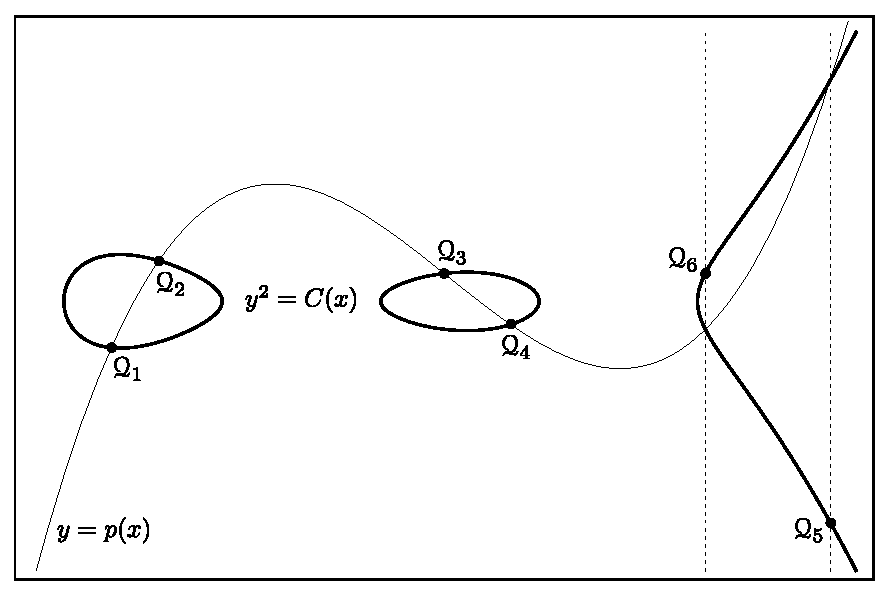
\includegraphics[width=0.9\textwidth]{addition_general.pdf}

		{\scshape Figure 1a}: The general case for the addition law in $\mathbbm{R}^2$ where $p_3 \neq 0$.

		\vspace{1mm}

		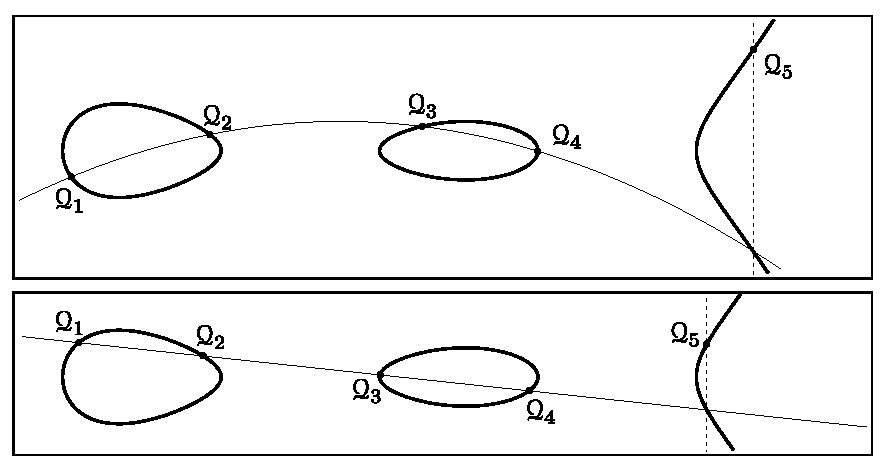
\includegraphics[width=0.9\textwidth]{addition_quadr_and_lin.pdf}

		{\scshape Figures 1b} and {\scshape 1c}: If $p_3 = 0$ we have at most five intersections.
	\end{center}
	\vspace{-1.5mm}
	\fline
\end{figure}

\vspace{2mm}
\begin{remark}
We will use this property extensively from now on and it will be worth the additional trouble of having to check well-definedness because
\begin{enumerate}[(i)]\parskip 0mm
	\item Since \eqref{switch} implies that we can interchange \textit{any} two point-components in a given sum, we may now impose conditions on the $\q_i$ without mentioning whether they belong to $\P_1$ or $\P_2$.
	\item As a result, the list of special cases can be written in a significantly more concise manner.
	\item It is immediately clear now that if we have a well-defined addition, then $-\P = \bar \P$ because $\{ \q_1 , \q_2 \} + \{ \bar \q_1 , \bar \q_2 \} = \{ \q_1 , \bar \q_1 \} + \{ \q_2 , \bar \q_2 \}=0$.
	\item The property even gives us commutativity for free.
\end{enumerate}
\parskip 3mm
\end{remark}

%xxx not 100\% satisfactory...I really want to show that this is not only justified but  inevitable.

\newpage
\subsection{Complete List of Cases}

As we strive to define $\{ \q_1 , \q_2 \} + \{ \q_3 , \q_4 \}$, for any $\q_i = (x_i,y_i) \in \enkb$ or $\q_i = \infty \in \ekb$ we observe that the following simplification takes place:

Let $\{ i,j,k,l \}=\{ 1,2,3,4 \}$. Whenever $\q_i = \bar \q_j$ for $i \neq j$ we define
\begin{align*}
  \{ \q_1 , \q_2 \} + \{ \q_3 , \q_4 \} &= \{ \q_k , \q_l \} + \{ \q_i , \bar \q_i \}\\
  &= \{ \q_k , \q_l \} + \{ \infty, \infty \}.
\end{align*}
The justification for this follows directly from \eqref{switch} and Definition \ref{defj}. It is easily checked that this sum remains well defined if the choice of $i$ and $j$ is not unique. This allows us to treat the above as a separate case in order to characterize the other cases solely through the $x$-coordinates of the $\q_i$, so% and otherwise xxx for all the others assume that equality between the $\q_i$ depend only on their $x$-coordinates:%any property we impose on the $\q_i$ we can just look at $x_i$:
\begin{align*}
  x_i = x_j \iff \q_i = \q_j
\end{align*}
for any $\q_i, \q_j \in \ekb$ provided we assign $\q_i = \infty$ the $x$-coordinate $x_i = \ii$.

We may now write the distinction between the remaining cases as follows:

\begin{enumerate}[A.]
	\parskip 1mm
	\item The general case where all $x_1,..,x_4$ are pairwise distinct.
	\item The case $x_i = x_j$ but $x_i$, $x_k$ and $x_l$ are pairwise distinct.
	\item The case where $x_i = x_j$ and $x_k = x_l$ but $x_i \neq x_k$.
	\item The case $x_i = x_j = x_k$ but $x_l \neq x_i$.
	\item The case where $x_1 = x_2 = x_3 = x_4$.
\end{enumerate}
\parskip 3mm

Since we are allowed to permute point-components anyway, we may fix which of the $\q_i$ are equal and write everything out for the complete and final list:

\vspace{-3mm}
\fline
% \vspace{-2mm}
\begin{enumerate}\setcounter{enumi}{-1}
	\parskip 1mm
	\item The addition with zero, i.e. $\P + \{ \infty, \infty \}$ or in short $\P + 0$, $\P \in \J$.
	\item The general case where all $\q_i$ in $\ek$ are pairwise distinct from $\pm \q_j$.
	\item The single tangential case where $\q_1 = \q_2 \in \enk$ with $y_1 \neq 0$ and the remaining $\q_3$, $\q_4 \in \ek$ are both distinct from each other as well as from $\pm \q_1, \bar \q_3$ and $\bar \q_4$.
	\item The double tangential case where $\q_1 = \q_2 \in \enk$ with $y_1 \neq 0$ and $\q_3 = \q_4 \in \enk$ with $y_3 \neq 0$ and $\q_1 \neq \pm \q_3$.
	\item The triple-point case wherein $\q_1=\q_2=\q_3 \in \enk$ with $y_1 \neq 0$ and $\q_4 \in \ek$ differs from both $\pm \q_1$.
	\item The quadruple case where all $\q_i \in \enk$ are equal with $y_i\neq 0$.
\end{enumerate}
\vspace{-2mm}
\fline
\parskip 3mm

\begin{remark}\label{rem}\hfill
\begin{enumerate}[(i)]
	\item In both lists, the cases do not overlap.
	
	\item For the list to be complete, we must allow for $\q_i = \infty$ for some $i$. Note that one is sufficient, since if two or more $\q_i$ were to be $\infty$, we would be back at the case 0 by virtue of \eqref{switch}, bringing the two infinities together in one point. As for case 1, we consider $\q_i \in \enk$ and $\q_i \in \ek$ in two separate cases and postpone handling the latter.\label{extend}

	\item As for the first case, the constructions will a priori only be made on $\j$. It remains to check that this makes indeed for a well-defined addition on $\J$ by being invariant under the permutations $\q_1 \rightleftharpoons \q_2$ and $\q_3 \rightleftharpoons \q_4$.
\end{enumerate}
\end{remark}

\subsection{Addition Law for the Special Cases}

\setcounter{case}{-1}

\begin{case}
  {\scshape Addition with Zero:} As one might have anticipated we define $\P_1 + \P_2 = \P_1$ for every $\P_1 \in \J$ if $\P_2 = \{\infty, \infty\} = 0$.
\end{case}

\setcounter{case}{1}
\begin{case}
	{\scshape Tangential:} Let $\q_i\in \enk, \q_1 = \q_2$, $y_1 \neq 0$ but $x_1$, $x_3$ and $x_4$ are pairwise distinct. We cannot use the Vandermonde matrix in this case because it won't possess maximal rank, consequently being non-invertible. We can however obtain an additional equation by demanding that our polynomial $p(x)$ be tangential to the curve at $\q_1$. This gives
	\begin{align*}
	  2 y \frac{dy}{dx} &= 5  x^4 + 4 a x^3 + 3 b x^2 + 2 c x + d \\
	  \text{and\hspace{8mm}} \frac{dy}{dx} &= 3 p_3 x^2 + 2 p_2 x + p_1
	\end{align*}
	meaning that the system to solve for $\mathbf{p}$ is now $\Vdoub \cdot \mathbf{p} = \ydoub$ with
	\begin{align*}\Vdoub=
		\begin{pmatrix}
			1 & x_1 & x_1^2 & x_1^3\\
			0 & 1 & 2 x_1 & 3 x_1^2\\
			1 & x_3 & x_3^2 & x_3^3\\
			1 & x_4 & x_4^2 & x_4^3\\
		\end{pmatrix}.
	\end{align*}
	The subscript indicates at which points the intersections have higher order.
	Here $\ydoub$ is defined as $\mathbf{y}$ with $y_2$ replaced by $y_2'=\frac{C'(x_1)}{2 y_1}$ where $C'(x)$ is the derivative of $C$ and $2y_1 \neq 0$ because char$(K) \neq 2$ and $y_1\neq 0$. Since $\det(\Vdoub) = (x_4-x_1)^2(x_3-x_1)^2(x_4-x_3)$ this fits neatly into our constraints by being non-zero exactly in the case where $x_1, x_3$ and $x_4$ are pairwise distinct.

	Once $p(x)$ is determined, step two will be entirely identical to the general case and we can again solve \eqref{dagger2} or \eqref{dagger} for $x_5$ or $x_5$ and $x_6$.

	%Now let $\q_4 = \infty$. As an analogue to case one and with the same constraints as above, the relevant matrix $\tilde V_1$ is again the upper-left $3 \times 3$ sub-matrix of $V_1$ and we solve $\tilde V_1 \cdot \mathbf{p} = \tilde \mathbf{y}_1$ for a three-element vector $\mathbf{p}$. Needless to say that $\tilde V_1$ is invertible and by obtaining $\mathbf{p}$ we can solve \eqref{daggerp} to get $x_5$ and $x_6$.
\end{case}

\begin{case}
	{\scshape Double Tangential:} Let $\q_i \in \enk$, $\q_1 = \q_2$ and $\q_3 = \q_4$ but $x_1 \neq x_3$ and $\q_i \neq \pm \q_i$ meaning that neither $y_1$ nor $y_3$ will be zero. As before, we lack equations for our linear system, requiring the use of a second tangential constraint. Replace the fourth row of $\Vdoub$ and $\ydoub$ exactly like we did for the second one: $y_4'=\frac{C'(x_3)}{2 y_3}$ and
	\begin{align*}\Vddoub=
		\begin{pmatrix}
			1 & x_1 & x_1^2 & x_1^3\\
			0 & 1 & 2 x_1 & 3 x_1^2\\
			1 & x_3 & x_3^2 & x_3^3\\
			0 & 1 & 2 x_3 & 3 x_3^2\\
		\end{pmatrix}.
	\end{align*}

	Now $\det(\Vddoub)=(x_3-x_1)^4$ and this is again different from zero precisely whenever $x_3 \neq x_1$, so as before solve $\Vddoub \cdot \mathbf{p} = \yddoub$ for $\mathbf{p}$, then \eqref{dagger} or \eqref{dagger2}.
\end{case}

\begin{case}
	{\scshape Triple Point:} Let $\q_i \in \enk , \q_1=\q_2=\q_3$ but $x_1 \neq x_4$ and $y_1 \neq 0$. We can thus see this as a third-order intersection and demand that the curve and the polynomial share a second-order derivative at $\q_1$:
	\begin{align*}\Vtri=
			\begin{pmatrix}
			1 & x_1 & x_1^2 & x_1^3\\
			0 & 1 & 2 x_1 & 3 x_1^2\\
			0 & 0 & 2 & 6x_1\\
			1 & x_4 & x_4^2 & x_4^3\\
		\end{pmatrix}.
	\end{align*}
	Here $\det(\Vtri)=2(x_4-x_1)^3$ and with this, define $\ytri$ by taking $\ydoub$ and replacing the third coordinate by $y_3'' = \frac{C''(x_1)}{2y_1}-\frac{(C'(x_1))^2}{4y_1^3}$ where $C''(x)$ is the second-order derivative of $C$. Again, apply the same procedure of the second steps of case 1 to find $\P_3$.

	%Again, consider $\q_4 = \infty$ and as before we obtain a new system $\tilde V_{13} \cdot \mathbf{p} = \tilde \mathbf{y}_{13}$. $\tilde V_{13}$ is the upper-left $3 \times 3$ sub-matrix of $V_{13}$, is invertible and leads to $p(x)$ which we use to solve \eqref{daggerp}.
\end{case}

\begin{case}
	{\scshape Quadruple Point:} Given the situation where $\q_i = \q_1 \in \enk$ for every $i$ with $y_1 \neq 0$, we use
	\begin{align*}\Vquad &=
		\begin{pmatrix}
			1 & x_1 & x_1^2 & x_1^3\\
			0 & 1 & 2 x_1 & 3 x_1^2\\
			0 & 0 & 2 & 6x_1\\
			0 & 0 & 0 & 6\\
		\end{pmatrix}
	\end{align*}
	which is invertible in all fields but those of characteristic 2 and 3.

	Here $\yquad$ is the same as $\ytri$ except for the last coordinate which should read
	\begin{align*}
		% y_4''' = \frac{1}{2y_0}\Big( C'''(x_0) - \frac{dy}{dx}\bigg|_{\q}\Big(\big(\frac{dy}{dx}\bigg|_{\q}\big)^2 - \frac{d^2y}{dx^2}\bigg|_{\q} \Big) \Big).
		y_4''' = \frac{C'''(x_1)}{2y_1}-\frac{3C'(x_1)C''(x_1)}{4y_1^3}+\frac{3(C'(x_1))^3}{8y_1^5}
	\end{align*}
	where $C'''(x)$ is the third-order derivative of $C$. Once more, we solve the linear system $\Vquad \cdot \mathbf{p}=\yquad$ and subsequently \eqref{dagger} or \eqref{dagger2} and we're done.
\end{case}
% \vspace{-4mm}
\begin{center}
$\sim$
\end{center}

  \textbf{Finally}, as noted in Remark \ref{rem}, \eqref{extend} we have yet to extend our definition from $\enk$ to $\ek$. Observe that this is only relevant for cases number two and four where we now consider $\q_4 = \infty$ as we did in {\scshape Step $1'$} of the general case. As an analogue to this, the relevant matrices $\tilde V_1$ and $\tilde V_{11}$ will be the upper-left $3 \times 3$ sub-matrices of their $\enk$-counterparts $V_1$ and $V_{11}$.

  In both cases we obtain a linear system of the form $\tilde V_{\ast} \cdot \mathbf{p} = \tilde \mathbf{y}_{\ast}$ for a three-element vector $\mathbf{p}$ and the vectors $\tilde \mathbf{y}_{1}$ and $\tilde \mathbf{y}_{11}$ are defined like their 4-element counterparts $\mathbf{y}_{1}$ and $\mathbf{y}_{11}$ with the last coordinate omitted.

  Both matrices $\tilde V_{\ast}$ are invertible and we therefore get a unique polynomial $p(x)$ wich we use to solve \eqref{daggerp}, obtaining $x_5$, $x_6$, $y_5=p(x_5)$ and $y_6=p(x_6)$ in $\bar K$ and we define $\{ \q_1 , \q_2\}+\{ \q_3 , \infty \} = \{ \q_5 , \q_6 \} = \{(x_5,-y_5),(x_6,-y_6)\}$.
  %Now let $\q_4 = \infty$. As an analogue to case one and with the same constraints as above, the relevant matrix $\tilde V_1$ is again the upper-left $3 \times 3$ sub-matrix of $V_1$ and we solve $\tilde V_1 \cdot \mathbf{p} = \tilde \mathbf{y}_1$ for a three-element vector $\mathbf{p}$. Needless to say that $\tilde V_1$ is invertible and by obtaining $\mathbf{p}$ we can solve \eqref{daggerp} to get $x_5$ and $x_6$.

\subsection{Well-Definedness of the Addition Law}

To check whether our addition is well defined on $\J$ in each of the cases, we have to consider the permutation of point-components $\q_i$ under the equivalence relation from Definition \ref{defj}. Furthermore, to claim that all possible cases are all covered, it is necessary to check the permutations under \eqref{switch}. Both cases can be combined into a single one by the following statement:

\textbf{Lemma:} In each given definition of `$+$', the result is invariant under the permutation $\q_i \rightleftharpoons \q_j$.

\begin{proof}
  Simultaneously interchanging $x_i \rightleftharpoons x_j$ and $y_i \rightleftharpoons y_j$ in our linear systems $V_{\ast} \cdot \mathbf{p} = \mathbf{y}_{\ast}$ has the effect of permuting the rows of $V_{\ast}$ and $\mathbf{y}_{\ast}$ and relabeling $(x_k,y_k)$ whenever $\q_k$ was equal to $\q_i$ or $\q_j$.% Observe that the relevant expressions $\det (V_{\ast})$ and $p_3$ are untouched by this manipulation.

  Consequently the resulting $p(x)$ doesn't change, so neither do any of the terms $T_{\ast}$. The three dagger equations remain unchanged as well, as can easily be checked at \eqref{dagger}, \eqref{dagger2} and \eqref{daggerp} which are invariant under $x_i \rightleftharpoons x_j$.

  Finally, the version of Step 2 we fall into remains the same, since it is only imposed by the distinction of $p_3$ being zero or not. %the variation of the dagger equation of Step 2.
\end{proof}




%Matrices, det invariant under perm, xxx The same can be said for the explicit expression of $p_3$ noted in the general case. 



%2. Invariance under $\q_1 \rightleftharpoons \q_3$. Note that combined with the above, this includes the permutation $\q_1 \rightleftharpoons \q_4$.

%\subsection{Closing Remarks}

%xxx double (and triple?) zeroes of \eqref{sex} 




% -----------------------------------------------------------------------------
% THIS IS THE END. MY ONLY FRIEND, THE END. OF EVERYTHING THAT STANDS, THE END.
% NO SADNESS NOR SURPRISE, THE END.
% CAN YOU PICTURE WHAT WILL BE? SO LIMITLESS AND FREE.
% -----------------------------------------------------------------------------
\end{document}